\documentclass{article}

\usepackage[german]{babel}
\usepackage{tikz}
\usetikzlibrary{positioning}
\usepackage[colorlinks=true, urlcolor=blue, linkcolor=black]{hyperref}
\usepackage[doublespacing]{setspace}
\usepackage{geometry}
  \geometry{
    a4paper,
    right=30mm,
    left=30mm
  }

\usepackage{amsmath}
\usepackage{listings}

\title{Vorhersage von Kredit-Ausfallwahrscheinlichkeiten mit neuronalen Netzen}
\author{Thomas Siskos}
\date{ }

\begin{document}
\begin{titlepage}
  \begin{center}

  
\includegraphics[scale=1.25]{hulogo.pdf} \par
  {\scshape\LARGE Humboldt Universit{\"a}t zu Berlin \par}

  {\scshape\Large Hausarbeit\par}

  {\huge\bfseries Vorhersage von Kredit-Ausfallwahrscheinlichkeiten mit neuronalen Netzen\par}

\vspace{1cm}

  {\Large\itshape Thomas Siskos (580726)\par}

  {\Large\scshape Datenanalyse II\par}

  \vfill
  Dozent: \par
  {\Large Dr. Sigmund~\scshape Klinke \par}
  \vfill
  {\large \today\par}
  \end{center}
\end{titlepage}

\tableofcontents
\listoftables
\listoffigures
\newpage
\section{Einleitung}

Die Ausfallwahrscheinlichkeit ist ein Begriff der Finanzen und beschreibt die Wahrscheinlichkeit, dass ein Kreditnehmer, innerhalb eines Zeitrahmens, nicht in der Lage sein wird seine Verpflichtungen zum vorher festgelegten Termin einzuhalten. Die m{\"o}glichst genaue Sch{\"a}tzung und Vorhersage eines solchen Ausfalls ist von entscheidender Bedeutung. Die Bepreisung von Verm{\"o}genswerten, das Einsch{\"a}tzen der Risiken von Krediten und Kreditportfolios sowie die Wertsch{\"a}tzung anderer Finanz-Produkte h{\"a}ngen ma{\ss}geblich von der Pr{\"a}zision der gesch{\"a}tzten Ausfallwahrscheinlichkeiten ab (Miao et al., 2008). Es gibt zwei wesentliche Denkschulen bei der Analyse von Kreditausf{\"a}llen, der markt-basierte und der statistische Ansatz. Die markt-basierte Art modelliert Kreditausf{\"a}lle mithilfe struktureller Modelle, wohingegen der statistische Ansatz empirische Methoden bem{\"u}ht, historische Daten auszuwerten. Diese Daten k{\"o}nnen beispielsweise aus der Buchhaltung, beziehungsweise aus den Bilanzen von Unternehmen gewonnen werden (H{\"a}rdle et al., 2012).

Zur Quantifizierung der Ausfallwahrscheinlichkeit werden in der Literatur oft Kennzahlen verwendet, die vornehmlich eine oder mehrere Bilanzpositionen gegen eine oder mehrere andere ins Verh{\"a}ltnis setzen. Diese Kennzahlen haben sich in vergangenen Studien oft als hilfreich erwiesen (Altman, 1968). In dieser Arbeit werden wir die 28 finanziellen Kennzahlen bestimmen, die von Zhang und H{\"a}rdle (2010) verwendet wurden. Wir werden mithilfe dieses transformierten Datensatzes neuronale Netze unterschiedlicher Architekturen trainieren und miteinander vergleichen. Insbesondere verwenden wir klassische neuronale Netze mit einer versteckten Schicht, Netze mit zwei versteckten Schichten und Netze mit f{\"u}nf versteckten Schichten. Au{\ss}erdem werden wir versuchen die Entscheidungsprozesse eines simplen neuronalen Netzes mithilfe von Konturenplots zu visualisieren und zu interpretieren. Die verschiedenen Architekturen wurden mithilfe der Programmiersprache \texttt{Python}, genauer mit dem Modul \texttt{tensorflow}, erzeugt. Der Quellcode f{\"u}r die neuronalen Netze ist auf \href{https://github.com/thsis/DAII}{github.com/thsis/DAII} einsehbar.

Der folgende Abschnitt beschreibt den Datensatz der Creditreform Datenbank, sowie die Art und Weise wie die Daten bereinigt und transformiert wurden um die 28 Finanz-Kennzahlen zu bestimmen. Abschnitt 3 erl{\"a}utert die Theorie und Anwendung neuronaler Netze auf die Daten. Der vierte Abschnitt pr{\"a}sentiert die Ergebnisse. Der letzte Abschnitt enth{\"a}lt eine abschlie{\ss}ende Zusammenfassung und kritische W{\"u}rdigung.

\begin{center}
\begin{table}
\centering
\caption{Variablen des Creditreform Datensatzes}
\label{creditVars}
\begin{tabular}{cc}
\hline\hline
Variable & Bedeutung\\
\hline
ID & Kennnummer jedes Unternehmens\\
T2 & Solvenz-Status (solvent:0, insolvent:1)\\
JAHR & Jahr\\
VAR1 & Scheck, Kassenbestand\\
VAR2 & Vorr{\"a}te - Gesamt\\
VAR3 & Umlaufverm{\"o}gen\\
VAR4 & Sachanlagen - Gesamt\\
VAR5 & Immaterielle Verm{\"o}gensbest{\"a}nde\\
VAR6 & Gesamtverm{\"o}gen\\
VAR7 & Forderungen aus Lieferung und Leistung\\
VAR29 & Forderungen gg{\"u}. Unternehmen mit Beteiligungsverh{\"a}ltnis\\
VAR8 & Grundst{\"u}cke und Bauten\\
VAR9 & Eigenkapital\\
VAR10 & Gesellschafterdarlehen\\
VAR11 & Pesionsr{\"u}ckstellungen \\
VAR12 & kurzfristige Verbindlichkeiten - Gesamt\\
VAR13 & langfristige Verbindlichkeiten - Gesamt\\
VAR14 & Bankschulden\\
VAR15 & Verbindlichkeiten aus Lieferung und Leistung\\
VAR30 & Verbindlichkeitern gg{\"u}. Unternehmen mit Beteiligungsverh{\"a}ltnis\\
VAR16 & Ums{\"a}tze\\
VAR17 & Vertriebs- / Verwaltungsaufwand\\
VAR18 & Abschreibungen\\
VAR19 & Zinsaufwendungen\\
VAR20 & Gewinn vor Zins und Steuern (EBIT)\\
VAR21 & Betriebsgewinn \\
VAR22 & Jahres{\"u}berschuss \\
VAR23 & (Lager-) Bestandsver{\"a}nderungen \\
VAR24 & Ver{\"a}nderungen der Verbindlichkeiten gg{\"u}. Vorjahr\\
VAR25 & Ver{\"a}nderungen Bargeld/Kassenbestand/fl{\"u}ssige Mittel\\
VAR26 & Branchenzugeh{\"o}rigkeit\\
VAR27 & Rechtsform\\
VAR28 & Anzahl Mitarbeiter\\
\hline\hline
\end{tabular}
\end{table}
\end{center}


\section{Die Creditreform Datenbank}

Die Creditreform Datenbank enth{\"a}lt Daten f{\"u}r 20.000 solvente und 1.000 insolvente deutsche Firmen aus den Jahren 1997 bis 2007. Der Datensatz wurde durch das Labor f{\"u}r empirische und quantitative Forschung (\href{https://leqr.wiwi.hu-berlin.de/leqr/content/databaseInformation/creditreform/creditreform.htm}{LEQR}) der Humboldt Universit{\"a}t zu Berlin bereitgestellt. Die enthaltenen Variablen stammen aus den Bilanzen der Unternehmen und stellen f{\"u}r potentielle Investoren die Hauptgrundlage f{\"u}r Analysen dar. Ein Unternehmen wird entweder mit sich selbst verglichen, indem der zeitliche Verlauf der Bilanzposten untersucht wird oder das Unternehmen wird mit {\"a}hnlichen Firmen verglichen, indem eine Auswahl finanzieller Kennzahlen betrachtet wird (Berk \& DeMarzo, 2016).

Rund die H{\"a}lfte der Daten stammt aus den Jahren 2001 und 2002. Da 1996 keine insolventen Unternehmen vorliegen, werden alle Beobachtungen dieses Jahres gel{\"o}scht. Der Gro{\ss}teil der verbleibenden Unternehmen ist entweder im Baugewerbe, im Handel, in der Industrue oder im Immobilienwesen t{\"a}tig. Andere Kategorien umfassen beispielsweise Branchen wie Landwirtschaft und Bergbau, Elektrizit{\"a}t-, Gas- und Wasserversorgung, die Gastronomie, Logistik und soziale Dienstleistungen. Alle Unternehmen die zu diesen Kategorien geh{\"o}ren werden von der folgenden Analyse ausgeschlossen, um die Schichtung des Trainingsdatensatzes nicht unn{\"o}tig zu komplizieren. Au{\ss}erdem werden sowohl die kleinsten, als auch die gr{\"o}{\ss}ten Unternehmen entfernt. Betrachtet werden nur Unternehmen, deren Gesamtverm{\"o}gen zwischen 10.000 und 10.000.000 Euro liegen. Die kleinsten Unternehmen werden entfernt, da deren finanzielle Lage oft von den Finanzen einer einzelnen verantwortlichen Person, typischerweise die Eigent{\"u}merin oder der Eigent{\"u}mer, abh{\"a}ngt. Die gr{\"o}{\ss}ten Unternehmen werden hingegen entfernt, da sie in Deutschland nur in den allerseltensten F{\"a}llen Gefahr laufen in die Zahlungsunf{\"a}higkeit zu geraten. Des Weiteren werden Unternehmen entfernt, bei denen w{\"a}hrend der Berechnung der finanziellen Kennzahlen Nullen im Nenner auftreten (Chen, 2010).

\begin{table}
\begin{center}
\centering
\caption{Definitionen der finanziellen Kennzahlen}
\scriptsize
\vspace{1mm}
\begin{tabular}{ccc}
\hline\hline
Name & Formel & Kennzahl \\
\hline
x1 & VAR22/VAR6 & Gesamtkapitalrentabilit{\"a}t (ROA) \\
x2 & VAR22/VAR16 & Nettogewinnmarge \\
x3 & VAR21/VAR6 & \\
x4 & VAR21/VAR16 & Betriebsgewinnmarge \\
x5 & VAR20/VAR6 & \\
x6 & (VAR20+VAR18)/VAR6 & EBITDA \\
x7 & VAR20/VAR16 & \\
x8 & VAR9/VAR6 & Eigenmittelquote (einfach)\\
x9 & (VAR9-VAR5)/(VAR6-VAR5-VAR1-VAR8) & Eigenmittelquote (angepasst) \\
x10 & VAR12/VAR6 & \\
x11 & (VAR12-VAR1)/VAR6 & Nettoverschuldung \\
x12 & (VAR12+VAR13)/VAR6 & \\
x13 & VAR14/VAR6 & Schuldenquote \\
x14 & VAR20/VAR19 & Zinsdeckungsgrad \\
x15 & VAR1/VAR6 & \\
x16 & VAR1/VAR12 & Liquidit{\"a}tsgrad \\
x17 & (VAR3-VAR2)/VAR12 & Quick Ratio \\
x18 & VAR3/VAR12 & Current Ratio \\
x19 & (VAR3-VAR12)/VAR6 & \\
x20 & VAR12/(VAR12+VAR13) & \\
x21 & VAR6/VAR16 & Kapitalumschlag \\
x22 & VAR2/VAR16 & Lagerumschlag \\
x23 & VAR7/VAR16 & Forderungsumschlag \\
x24 & VAR15/VAR16 & Verbindlichkeitenumschlag \\
x25 & log(VAR6) & Proxy f{\"u}r die Unternehmensgr{\"o}{\ss}e \\
x26 & VAR23/VAR2 & Gestaffelte Prozentuale Lagerbestands{\"a}nderung \\
x27 & VAR24/(VAR12+VAR13) & Gestaffelte Prozentuale Forderungs{\"a}nderung \\
x28 & VAR25/VAR1 & Gestaffelte Prozentuale {\"a}nderung des Cash Flow \\
\hline\hline
\end{tabular}
\end{center}
\end{table}


Die verbleibenden Unternehmen gliedern sich in verschiedene Sektoren, von denen die vier h{\"a}ufigsten im Folgenden analysiert werden. Von den 9567 solventen Unternehmen sind 35,9\% in der Industrie, 34,1\% im Handel, 19,5\% im Baugewerbe und 10,4\% in der Immobilienbranche t{\"a}tig. Von den 782 insolventen Unternehmen sind 45,0\% im Baugewerbe, 28,2\% in der Industrie, 21,6\% im Handel und 5,1\% in der Immobilienbranche t{\"a}tig.

Anschlie{\ss}end werden mithilfe der verbleibenden Unternehmen die finanziellen Kennzahlen ermittelt. Die Variablen \texttt{x1}-\texttt{x7} geh{\"o}ren zu den sogenannten Rentabilit{\"a}tsverh{\"a}ltnissen. Rentabilit{\"a}tsverh{\"a}ltnisse haben sich in der Vergangenheit als besonders starke Pr{\"a}diktoren f{\"u}r Kreditausf{\"a}lle erwiesen. Zum Beispiel gew{\"a}hrt die Gesamtkapitalrentabilit{\"a}t (return on assets, ROA) \texttt{x1} einen Einblick in die Umsatzst{\"a}rke eines Unternehmens im Vergleich zu dessen Kosten. So signalisiert ein h{\"o}herer Wert der Kennzahl, dass ein Unternehmen in der Lage ist mehr Geld mit weniger Mitteln zu verdienen. Die Nettogewinnmarge \texttt{x2} hingegen veranschaulicht den Anteil des Umsatzes, den das Unternehmen als Einnahmen einbeh{\"a}lt. Ein hoher Wert geht mit einem profitablen Unternehmen einher, das seine Kosten zu kontrollieren versteht (Chen et al., 2011).

Eine weitere Reihe der Kennzahlen beschreibt die sogenannte Hebelwirkung. Damit ist das Ausma{\ss} gemeint, in dem ein Unternehmen auf Schulden als Finanzierungsquelle angewiesen ist (Berk \& DeMarzo, 2016). Da Unternehmen Schulden und Eigenkapital kombinieren, um ihre Aktivit{\"a}ten zu finanzieren, erweisen sich Kennzahlen {\"u}ber ebenjene Hebelwirkung als hilfreiche Werkzeuge um die Zahlungsf{\"a}higkeit eines Unternehmens einzusch{\"a}tzen. Zu den Kennzahlen der Hebelfinanzierung geh{\"o}ren die Variablen \texttt{x8}-\texttt{x14}. Beispielsweise misst die Nettoverschuldung \texttt{x11} die H{\"o}he der kurzfristigen Verpflichtungen, welche nicht durch die liquidesten Verm{\"o}gensbest{\"a}nde gedeckt sind, als prozentualer Anteil des Gesamtverm{\"o}gens. Somit misst diese Kennzahl auch die kurzfristige Liquidit{\"a}t eines Unternehmens (Chen et al., 2011).

Die sechs Folgenden Verh{\"a}ltnisse \texttt{x15}-\texttt{x20} geh{\"o}ren in den Bereich der Liquidit{\"a}ts-Kennzahlen. Liquidit{\"a}t ist eine weit verbreitete Variable, die in vielen Kreditentscheidungen eine wichtige Rolle spielt. Liquidit{\"a}t beschreibt die M{\"o}glichkeiten eines Unternehmens Verm{\"o}gensbest{\"a}nde in kurzer Zeit in Bargeld umzuwandeln. Die wohl wichtigste Kennzahl f{\"u}r die Liquidit{\"a}t ist der Anteil der Kassenbest{\"a}nde am Gesamtverm{\"o}gen \texttt{x15}. Ein weiterer wichtiger Gradmesser f{\"u}r die Liquidit{\"a}t eines Unternehmens ist der sogenannte Quick-Ratio \texttt{x17}. Mithilfe des Quick-Ratio versucht man einzusch{\"a}tzen, ob ein Unternehmen {\"u}ber ausreichend liquide Mittel verf{\"u}gt um insbesondere kurzfristige Zahlungen zu decken. Ein hoher Quick-Ratio indiziert, dass es f{\"u}r das Unternehmen unwahrscheinlich ist, kurzfristig in Zahlungsnot zu geraten (Berk \& DeMarzo, 2016).

Einen weitereren wichtigen Typus von betriebswirtschaftlichen Kennzahlen stellen die Aktivit{\"a}tskennzahlen \texttt{x21}-\texttt{x24} dar. Aktivit{\"a}tskennzahlen messen die Effizienz mit der ein Unternehmen eigene Ressourcen aufwendet, um Umsatz mithilfe seiner Verm{\"o}gensbest{\"a}nde zu generieren (Chen et al., 2011).

Zus{\"a}tzlich berechnen wir den Logarithmus des Gesamtverm{\"o}gens \texttt{x25}. Dieser Risikoindikator stellt die Gr{\"o}{\ss}e eines Unternehmens dar und versetzt uns in die Lage gro{\ss}e, mittlere und kleine Unternehmen miteinander in Beziehung zu setzen. Als letzte Gruppe betriebswirtschaftlicher Kennzahlen berechnen wir die gestaffelten prozentualen {\"a}nderungen des Cash-Flow, des Lagerbestandes und der Forderungen im Vergleich zum Vorjahr \texttt{x26}-\texttt{x28}. (Chen et al., 2011).

Um Einfl{\"u}sse von Ausrei{\ss}ern auf die neuronalen Netze zu eliminieren, werden extreme Werte f{\"u}r die verschiedenen Verh{\"a}ltnisse durch das 0.05- bzw. das 0.95-Quantil ersetzt. Pr{\"a}ziser ausgedr{\"u}ckt, folgen wir der Regel, wenn $x_{ij} < q_{0.05}(x_j)$, dann setze $x_{ij} \stackrel{!}{=} q_{0.05}(x_j)$. Beziehungsweise, wenn $x_{ij} > q_{0.95}(x_j)$, dann setze $x_{ij} \stackrel{!}{=} q_{0.95}(x_j)$. Wobei $x_i, i \in \{1, \vdots, N\}$ f{\"u}r jeden einzelnen Wert einer Kennzahl $x_j$ und $q_k(x_j), j \in \{1, \vdots, 28\}, k=0.05, 0.95$ f{\"u}r die jeweiligen Quantile der Kennzahl $x_j$ des Datensatzes steht.

\section{Methoden}
\subsection{Neuronale Netze}

K{\"u}nstliche neuronale Netze versuchen die Struktur von Gehirnen nachzubilden. Stark vereinfacht enth{\"a}lt ein jedes Gehirn sogenannte Neuronen, welche {\"u}ber zwei Zust{\"a}nde verf{\"u}gen k{\"o}nnen. Ein Neuron ist entweder aktiviert oder nicht. In einem Gehirn ver{\"a}ndern Neuronen ihren Zustand als Reaktion auf einen chemischen oder elektrischen Stimulus. Das Netz, das die Neuronen innerhalb des Gehirns eines Menschen bilden ist ein enormes Gespinst, in dem der Zustand eines Neurons das Ergebnis tausender anderer Neuronen sein kann. F{\"u}hrt ein Stimulus dazu, dass bestimmte Verbindungen wiederholt aktiviert werden, verfestigt sich deren Verbindung. Das f{\"u}hrt dazu, dass bei einem {\"a}hnlichen Stimulus ebenfalls dieselben Verbindungen aktiviert werden und zu demselben Outputzustand f{\"u}hren. Dieses Verhalten nennen wir Lernen (Duda, 2012).

K{\"u}nstliche neuronale Netze vereinfachen die Vorg{\"a}nge des Gehirns stark. Ein k{\"u}nstliches Neuron wird durch eine Aktivierungsfunktion simuliert, deren Bildmenge das Verhalten eines Schalters emuliert. Wir verlangen von der Aktivierungsfunktion, dass sie {\"u}ber mindestens zwei deutlich verschiedene Zust{\"a}nde verf{\"u}gt. Typischerweise ist der Output einer Aktivierungsfunktion zum Beispiel entweder Null oder Eins, Null oder gr{\"o}{\ss}er Null, Minus Eins oder Eins oder eine sigmoidale Funktion, welche auf dem Intervall $ \left[0, 1\right] $ beschr{\"a}nkt ist. Die Aktivierungsfunktion die in der folgenden Analyse verwendet wird besitzt die Form

\begin{equation}
\label{sigmoid}
\phi (z) = \frac{1}{1 + \exp (-z)}.
\end{equation}

Wie bereits erl{\"a}utert wurde, sind biologische Neuronen Teil eines hierarchischen Netzwerkes, in dem das Signal von manchen in andere Neuronen eingespeist wird. Im Allgemeinen wird diese Struktur durch miteinander verbundene \textit{Knoten} einer \textit{Schicht} repr{\"a}sentiert. Ein Netzwerk besteht aus einer Input, ein oder mehrerer versteckter Schichten und einer Output-Schicht. Der Name der mittleren Schichten tr{\"a}gt der Tatsache Rechnung, dass das Wirken der versteckten Schichten zu einem gewissen Grad nur schwer zu beobachten, zuweilen sogar komplett unbeobachtbar ist. F{\"u}r gew{\"o}hnlich sieht der Benutzer eines neuronalen Netzes nur das, was eingespeist wird, sowie dessen Ergebnis. Innerhalb eines \textit{Knoten} wird die Aktivierungsfunktion des Neurons auf die gewichtete Summe aller Kanten des Graphen angewandt. Der Output $h^{k}_l$ eines \textit{Knoten} der ersten versteckten Schicht $H^{(1)}_l$ ist somit als

\begin{equation}
\label{nodeOut}
\begin{split}
h^{(k)}_l &= \phi(\beta_0 + x_1 \beta_1 + \dots + x_{28} \beta_{28}) \\
        &= \frac{1}{1 + \exp (-\beta_0 - \beta_1 w_1 - \dots - \beta_{28}x_{28})}.
\end{split}
\end{equation}


\tikzset{
  every neuron/.style={
    circle,
    draw,
    minimum size=1cm},
  neuron missing/.style={
    draw=none,
    scale=3,
    text height=0.333cm,
    execute at begin node=\color{black}$\vdots$},
}

\begin{figure}
\centering
\caption{Neuronales Netz mit einer versteckten Schicht.}
\label{NN1L}
\vspace{2mm}
\begin{tikzpicture}[x=1.5cm, y=1.5cm, >=stealth]
% plot input layer
\foreach \m/\1 [count=\y] in {1, 2, missing, 3}
  \node [every neuron/.try, neuron \m/.try] (input-\m) at (0, 2.5-\y) {};

\foreach \m [count=\y] in {1, missing, 2}
  \node [every neuron/.try, neuron \m/.try] (hidden-\m) at (2, 2-\y*1.1) {};

\foreach \m [count=\y] in {1}
  \node [every neuron/.try, neuron \m/.try] (output-\m) at (4, 0) {};

\foreach \l [count=\i] in {1,2,28}
  \draw [<-] (input-\i) -- ++(-1,0)
    node [above, midway] {$X_{\l}$};

\foreach \l [count=\i] in {1}
  \draw [->] (output-\i) -- ++ (1,0)
    node [above, midway] {$O_\i$};

\foreach \l [count=\i] in {1, 10}
  \node [above] at (hidden-\i.north) {$H^{(1)}_{\l}$};

\foreach \i in {1, 2, 3}
  \foreach \j in {1,2}
    \draw [->] (input-\i) -- (hidden-\j);

\foreach \i in {1, 2}
  \draw [->] (hidden-\i) -- (output-1);


\foreach \l [count=\x from 0] in {Input-, Versteckte, Output-}
  \node [align=center, above] at (\x*2,2) {\l \\ Schicht};
\end{tikzpicture}
\end{figure}

Das Signal $o_1$ des Output-Knotens $O_1$ ist wiederum eine gewichtete Summe der Outputs der versteckten Schicht (Duda, 2012).

\begin{equation}
\label{outOut}
o_1 = \phi \left(\sum_{q=0}^{u} \gamma_q h^{(1)}_q\right)
\end{equation}

Mithilfe dieser Gleichungen lassen sich die Inputs vorw{\"a}rts durch das Netzwerk propagieren, vorausgesetzt man kennt die Gewichte $\beta$ und $\gamma$. Im Allgemeinen muss man die Gewichte zun{\"a}chst ermitteln. Dies geschieht durch die Optimierung einer Kostenfunktion. Im Falle bin{\"a}rer Zustandsvariablen bietet sich die Kreuzentropie an (Duda, 2012).

\begin{equation}
\label{crossEnt}
J = - \frac{1}{n} \sum \left( y \log a + (1-y) \log(1-a) \right),
\end{equation}

wobei $a$ f{\"u}r die jeweilige Aktivierungsfunktion steht (Duda, 2012).

Die Kreuzentropie aus Gleichung \ref{crossEnt} vereint zwei Eigenschaften, die sie als Kostenfunktion besonders auszeichnen. Sie ist gr{\"o}{\ss}er Null und wenn der Output $a$ des Endknotens nahe am tats{\"a}chlichen Zustand der Beobachtung liegt, ist der Wert des Summanden an dieser Stelle ebenfalls sehr gering. F{\"u}r die optimalen Gewichte gilt es, $J$ zu minimieren. Das Verfahren dazu nennt sich in der Literatur \textit{backpropagation} und ist eine Anwendung der Kettenregel des Ableitens.

\begin{equation}
\label{backProp}
\begin{split}
\frac{\partial J}{\partial \beta_j} &= - \frac{1}{n}\sum \left( \frac{y}{\sigma (z)} - \frac{1-y}{1-\sigma(z)}
                                      \right) \frac{\partial \sigma}{\partial \beta_j} \\
                                    &= - \frac{1}{n}\sum \left( \frac{y}{\sigma (z)} - \frac{1-y}{1-\sigma(z)}
                                      \right) \sigma(z) \left( 1- \sigma(z) \right) x_j .
\end{split}
\end{equation}

Wobei wir die sigmoidale Aktivierungsfunktion $\sigma(z)$ f{\"u}r $a$ in Gleichung \ref{crossEnt} eingesetzt haben. Gleichung \ref{backProp} l{\"a}sst sich weiter vereinfachen,
\begin{equation}
\label{backProp2}
\begin{split}
\frac{\partial J}{\partial \beta_j} &= \frac{1}{n} \sum \frac{\sigma(z) \left( 1- \sigma(z)\right) x_j}{\sigma(z) \left( 1- \sigma(z) \right)} \left( \sigma(z) - y \right) \\
                                    &= \frac{1}{n} \sum x_j \left( \sigma(z) - y \right) \stackrel{!}{=} 0 .
\end{split}
\end{equation}

Der Ausdruck in \ref{backProp2} besagt, dass die Rate mit der das Gewicht gelernt wird, von dem Fehler in $\left( \sigma(z) - y \right)$ abh{\"a}ngt. Je gr{\"o}{\ss}er dieser Fehler, desto schneller lernt das Neuron.



\subsection{Architekturen und Hyperparameter}

Im Folgenden stellen wir kurz den Aufbau der verwendeten neuronalen Netze vor. Es wurden drei verschiedene Architekturen implementiert, die erste enth{\"a}lt genau eine versteckte Schicht, genau wie in Abbildung \ref{NN1L}. Die zweite Art Netz, dargestellt in Abbildung \ref{NN2L}, enth{\"a}lt zwei versteckte Schichten und die dritte Architektur, dargestellt in Abbildung \ref{fiveLayers}, beherbergt f{\"u}nf versteckte Schichten. Bei allen neuronalen Netzwerken handelt es sich um sogenannte \textit{feed-forward-networks}. Das bedeutet, dass die beobachteten Daten von links nach rechts durch das Netzwerk propagiert werden. Alle Neuronen sind vollst{\"a}ndig miteinander verbunden. Falls mehrere Schichten vorhanden sind, sind diese jeweils symmetrisch aufgebaut, das hei{\ss}t alle versteckten Schichten enthalten jeweils dieselbe Anzahl an Neuronen.

Es werden drei Hyperparameter verwendet. Der markanteste ist sicherlich die Anzahl an Neuronen, da davon die gesamte Struktur der jeweiligen neuronalen Netze abh{\"a}ngt. F{\"u}r alle drei Architekturen wird zuerst ein Netz trainiert, das jeweils ein Neuron pro versteckter Schicht enth{\"a}lt, anschlie{\ss}end werden Netze trainiert deren Schichten zehn Neuronen enthalten und abschlie{\ss}end werden Netze trainiert deren Schichten zwanzig Neuronen enthalten.

\begin{table}
\begin{center}
\centering
\caption{Verwendete Hyperparameter}
\vspace{1mm}
\begin{tabular}{cccc}
\hline\hline
Hyperparamter & Verwendete Werte & \\
\hline
Anzahl Neuronen & 1 & 10 & 20 \\
Lern-Rate       & 0.01 & 0.005 & \\
Epochen & 10.000 & 100.000 & \\
\hline
\end{tabular}
\end{center}
\end{table}

Um die Kostenfunktion zu optimieren, wurde ein Gradientenverfahren angewandt, dessen Lern-Rate einmal $0.01$ und $0.005$ betrug. Es wurden jeweils einmal 10.000 und 100.000 Trainingsschritte unternommen. Insgesamt wurden somit 36 Modelle trainiert. Um die G{\"u}te der Vorhersagen zu quantifizieren wurden sogenannte \textit{Receiver-Operator-Characteristic (ROC)} Kurven gezeichnet sowie die Fl{\"a}che unter den jeweiligen Kurven (AUC) berechnet.

\begin{figure}
\centering
\caption{Neuronales Netz mit zwei versteckten Schichten.}
\label{NN2L}
\vspace{2mm}
\begin{tikzpicture}[x=1.5cm, y=1.5cm, >=stealth]
\foreach \m/\1 [count=\y] in {1, 2, missing, 3}
  \node [every neuron/.try, neuron \m/.try] (input-\m) at (0, 2.5-\y) {};

\foreach \m [count=\y] in {1, missing, 2}
  \node [every neuron/.try, neuron \m/.try] (hidden1-\m) at (2, 2-\y*1.1) {};

\foreach \m [count=\y] in {1, missing, 2}
  \node [every neuron/.try, neuron \m/.try] (hidden2-\m) at (4, 2-\y*1.1) {};

\foreach \m [count=\y] in {1}
  \node [every neuron/.try, neuron \m/.try] (output-\m) at (6, 0) {};

\foreach \l [count=\i] in {1,2,28}
  \draw [<-] (input-\i) -- ++(-1,0)
    node [above, midway] {$X_{\l}$};

\foreach \l [count=\i] in {1}
  \draw [->] (output-\i) -- ++ (1,0)
    node [above, midway] {$O_\i$};

\foreach \l [count=\i] in {1, 10}
  \node [above] at (hidden1-\i.north) {$H^{(1)}_{\l}$};

\foreach \l [count=\i] in {1, 10}
  \node [above] at (hidden2-\i.north) {$H^{(2)}_{\l}$};

\foreach \i in {1, 2}
  \foreach \j in {1,2}
    \draw [->] (hidden1-\i) -- (hidden2-\j);

\foreach \i in {1, 2}
  \draw [->] (hidden2-\i) -- (output-1);

\foreach \i in {1, 2, 3}
  \foreach \j in {1,2}
    \draw [->] (input-\i) -- (hidden1-\j);

\foreach \l [count=\x from 0] in {Input-, Erste Versteckte, Zweite Versteckte, Ouput-}
  \node [align=center, above] at (\x*2,2) {\l \\ Schicht};
\end{tikzpicture}
\end{figure}


Die ROC-Kurve wird ermittelt, indem man auf Basis der gesch{\"a}tzten Wahrscheinlichkeiten eines Test-Datensatzes Vorhersagen trifft. Diese Vorhersagen werden in die vier Felder einer sogenannten Konfusionsmatrix eingeordnet. Die Vorhersage kann entweder zutreffen, das hei{\ss}t einem Unternehmen wurde vorhergesagt, dass es nicht in der Lage sein wird einen Kredit zu bedienen und es ist tats{\"a}chlich nicht in der Lage (TP). Beziehungsweise es wird korrekterweise vorhergesagt, dass es solvent sein wird (TN). Oder die Vorhersage trifft nicht ein, einem solventen Unternehmen wurde die Insolvenz vorhergesagt (FP), beziehungsweise einem insolventen Unternehmen wurde f{\"a}lschlicherweise die Kreditw{\"u}rdigkeit vorhergesagt (FN). Damit sind alle m{\"o}glichen F{\"a}lle ersch{\"o}pft. Aus dieser Einteilung lassen sich die Falsch-Positiv-Rate (FPR), der Anteil aller f{\"a}lschlichen positiven Vorhersagen von allen eingetroffenen negativen Ausg{\"a}ngen

\begin{equation}
FPR = \frac{FP}{FP + TN}
\end{equation}

und die Sensitivit{\"a}t (TPR), das Verh{\"a}ltnis aller wahren positiven Vorhersagen und aller positiven Ausg{\"a}nge berechnen

\begin{equation}
TPR = \frac{TP}{TP + FN}.
\end{equation}

Die Fl{\"a}che unter der Kurve ist ein Ma{\ss} f{\"u}r die Vorhersagekraft eines Modells, wobei ein perfektes Modell einen AUC-Wert von eins annimmt. Ein AUC-Wert von 0.5 hingegen besagt, dass das Modell dieselbe pr{\"a}diktive Kraft besitzt, wie der Wurf einer fairen M{\"u}nze (Winkelmann, 2006).


\begin{figure}
\centering
\caption{Neuronales Netz mit f{\"u}nf versteckten Schichten.}
\label{fiveLayers}
\vspace{2mm}
\begin{tikzpicture}[x=1.5cm, y=1.5cm, >=stealth]
% input
\foreach \m/\1 [count=\y] in {1, 2, missing, 3}
  \node [every neuron/.try, neuron \m/.try] (input-\m) at (0, 2.5-\y) {};

\foreach \m [count=\y] in {1, missing, 2}
  \node [every neuron/.try, neuron \m/.try] (hidden1-\m) at (1, 2-\y*1.1) {};

\foreach \m [count=\y] in {1, missing, 2}
  \node [every neuron/.try, neuron \m/.try] (hidden2-\m) at (2, 2-\y*1.1) {};

\foreach \m [count=\y] in {1, missing, 2}
  \node [every neuron/.try, neuron \m/.try] (hidden3-\m) at (3, 2-\y*1.1) {};

\foreach \m [count=\y] in {1, missing, 2}
  \node [every neuron/.try, neuron \m/.try] (hidden4-\m) at (4, 2-\y*1.1) {};

\foreach \m [count=\y] in {1, missing, 2}
  \node [every neuron/.try, neuron \m/.try] (hidden5-\m) at (5, 2-\y*1.1) {};


\foreach \m [count=\y] in {1}
  \node [every neuron/.try, neuron \m/.try] (output-\m) at (6, 0) {};

\foreach \l [count=\i] in {1,2,28}
  \draw [<-] (input-\i) -- ++(-1,0)
    node [above, midway] {$X_{\l}$};

\foreach \l [count=\i] in {1}
  \draw [->] (output-\i) -- ++ (1,0)
    node [above, midway] {$O_\i$};

% names of hidden units
\foreach \j in {1, 2, 3, 4, 5}
  \foreach \l [count=\i] in {1, 10}
    \node [above] at (hidden\j-\i.north) {$H^{(\j)}_{\l}$};

% edges between hidden units
\foreach \i in {1, 2}
  \foreach \j in {1,2}
    \draw [->] (hidden1-\i) -- (hidden2-\j);

\foreach \i in {1, 2}
  \foreach \j in {1,2}
    \draw [->] (hidden2-\i) -- (hidden3-\j);

\foreach \i in {1, 2}
  \foreach \j in {1,2}
    \draw [->] (hidden3-\i) -- (hidden4-\j);

\foreach \i in {1, 2}
  \foreach \j in {1,2}
    \draw [->] (hidden4-\i) -- (hidden5-\j);

% last edge from 5th hidden layer to output
\foreach \i in {1, 2}
  \draw [->] (hidden5-\i) -- (output-1);

\foreach \i in {1, 2, 3}
  \foreach \j in {1,2}
    \draw [->] (input-\i) -- (hidden1-\j);

\foreach \l [count=\x from 0] in {Input-, Versteckte, Ouput-}
  \node [align=center, above] at (\x*3,2) {\l \\ Schicht(en)};
\end{tikzpicture}
\end{figure}


\section{Ergebnisse}

Die einzelnen Modelle wurden anhand eines Testdatensatzes beurteilt. Vor dem Training wurde der gesamte Datensatz nach dem Solvenzstatus der Beobachtungen getrennt. Der gesamte Datensatz enth{\"a}lt eine viel gr{\"o}{\ss}ere Anzahl solventer, als insolventer Unternehmen. Daher wurde zun{\"a}chst der kleinere Teildatensatz der insolventen Unternehmen im Verh{\"a}ltnis vier zu eins aufgeteilt. Diese beiden Datens{\"a}tze stellen jeweils die H{\"a}lfte des Trainings- und Testdatensatz dar. Anschlie{\ss}end wurde aus dem Teildatensatz der solventen Unternehmen zuf{\"a}llig Beobachtungen gezogen, so dass das Verh{\"a}ltnis von solventen und insolventen Firmen in Trainings- und Testdatensatz eins zu eins besteht.

\subsection{Eine versteckte Schicht}

Die AUC-Werte der verschiedenen Netze sind weitestgehend mittelm{\"a}{\ss}ig, wie Abbildung \ref{rocNN1L} zeigt. Die meisten liegen im Intervall zwischen 0.74 und 0.76. Dabei gibt es ein Modell, welches einen Wert von 0.5 aufweist und somit {\"u}ber {\"u}berhaupt keine Vorhersagekraft verf{\"u}gt. Das schlechteste Modell enthielt ein einziges Neuron in seiner Schicht und wurde mit der h{\"o}heren Lern-Rate von 0.01 {\"u}ber 100.000 Epochen trainiert. Ein Blick auf die Vorhersagen von Modell \texttt{nn1l8} verr{\"a}t, dass es lediglich den Mittelwert vorhersagt. Die besten aller einfachen Modelle, \texttt{nn1l6} und \texttt{nn1l10} enthielten jeweils 20 und 10 Neuronen in ihrer versteckten Schicht und wurden 100.000 Epochen lang trainiert. Modell \texttt{nn1l6} wurde mit der geringeren Lern-Rate von 0.005 gefittet, wohingegen die Lern-Rate f{\"u}r Modell \texttt{nn1l10} 0.01 betrug.

\begin{center}
\begin{figure}[h]
\caption{Entscheidungsgrenzen des einfachen Netzwerkes}
\label{NN1Linside}
\includegraphics[width=4.9cm]{../models/nn1l/nn1l_9/nn1l9_3_.png}
\includegraphics[width=4.9cm]{../models/nn1l/nn1l_9/nn1l9_0_.png}
\includegraphics[width=4.9cm]{../models/nn1l/nn1l_9/nn1l9_11_.png}
\end{figure}
\end{center}


\begin{center}
\begin{figure}[ht]
\centering
\caption{ROC-Kurve Neuronaler Netze mit einer versteckten Schicht}
\label{rocNN1L}
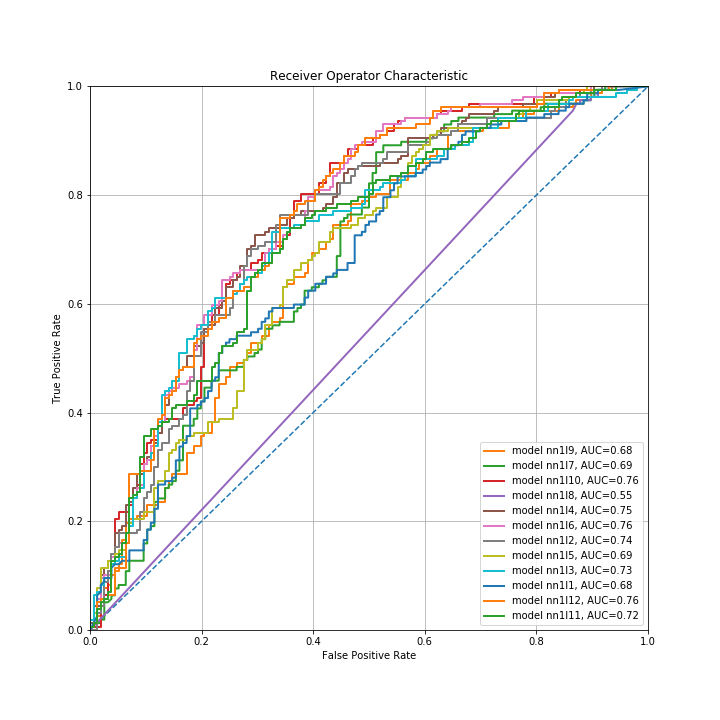
\includegraphics[width=15cm, height=13cm]{../rocNN1L.png}
\end{figure}
\end{center}


Exemplarisch stellen wir in Abbildung \ref{NN1Linside} einen Blick in das Innenleben der einfachen neuronalen Netze vor. Die Grafiken wurden erstellt, indem Vorhersagen f{\"u}r fiktive Datens{\"a}tze generiert wurden, in denen lediglich zwei Variablen manipuliert wurden. F{\"u}r diesen Datensatz wurden die Ausfallwahrscheinlichkeiten mithilfe des Modells \texttt{nn1l9} berechnet und die Kontouren der entstandenen dreidimensionalen Mannigfaltigkeit eingef{\"a}rbt und eingetragen.

In der linken Abbildung wurde die Betriebsgewinnmarge \texttt{x4} auf der Abszisse und der Quick-Ratio \texttt{17} auf der Ordinate abgetragen. Die F{\"a}rbung suggeriert, dass es ein Intervall innerhalb der Werte des Quick-Ratio gibt, welches das Risiko eines Kreditausfalls erh{\"o}ht und au{\ss}erhalb dessen es sich verringert. Dieser Effekt sollte jedoch nicht {\"u}berbewertet werden, da die Spannweite der vorhergesagten Ausfallwahrscheinlichkeiten lediglich von ca. 13 bis 25 Prozent reicht. Vielmehr soll mit dieser Abbildung gezeigt werden, dass selbst das simple neuronale Netzt in der Lage ist h{\"o}chst nichtlineare Zusammenh{\"a}nge aufzugreifen.

In der mittleren Abbildung wurde die Gesamtkapitalrentabilit{\"a}t \texttt{x1} gegen die Zinsdeckung \texttt{x14} abgetragen. Kurioserweise scheint die Betriebsgewinnmenge keinen Einfluss auf das vorhergesagte Ausfallrisiko zu haben, was man an den fast horizontal verlaufenden Konturen ablesen kann. Hingegen verringert sich das Ausfallrisiko je h{\"o}her die Zinsdeckung eines Unternehmens ausf{\"a}llt.

Die rechte Abbildung enth{\"a}lt die Konturen des Ausfallsrisikos, die man erh{\"a}lt, wenn man den Proxy f{\"u}r die Gr{\"o}{\ss}e eines Unternehmens \texttt{x25} gegen die Variable \texttt{x12} abtr{\"a}gt. Der Verlauf der Konturen legt Nahe, dass kleinere Unternehmen anf{\"a}lliger f{\"u}r Kreditausf{\"a}lle sind als gro{\ss}e, was auch der oben beschriebenen Intuition entspricht.

\subsection{Zwei versteckte Schichten}

Auch f{\"u}r zwei versteckte Schichten sehen die Werte der AUC-Metrik bestenfalls mittelm{\"a}{\ss}ig aus. Im Vergleich mit den einfachen Netzen f{\"a}llt jedoch auf, dass anteilig mehr Modelle die 0.7-Marke {\"u}berschreiten. Allerdings gibt es auch mehr Modelle, die durch eine schlechte Performanz auffallen. Das schlechteste aller Modelle \texttt{nn2l13} produziert Vorhersagen, bei denen es ratsam w{\"a}re das genaue Gegenteil der Vorhersage anzunehmen. Das Modell enthielt ein Neuron pro versteckter Schicht und wurde 10.000 Epochen lang mit einer besonders geringen Lern-Rate trainiert. Die Vermutung liegt nahe, dass der Trainingsprozess vorzeitig abgebrochen wurde und dass somit ein Fall von \textit{underfitting} vorliegt. Das beste Modell enthielt je zwanzig Neuronen pro Schicht. Die Trainings-Schleife wurde mit einer Lern-Rate von 0.01 {\"u}ber 100.000 Epochen durchlaufen.

\begin{center}
\begin{figure}[ht]
\centering
\caption{ROC-Kurve Neuronaler Netze mit zwei versteckten Schichten}
\label{rocNN2L}
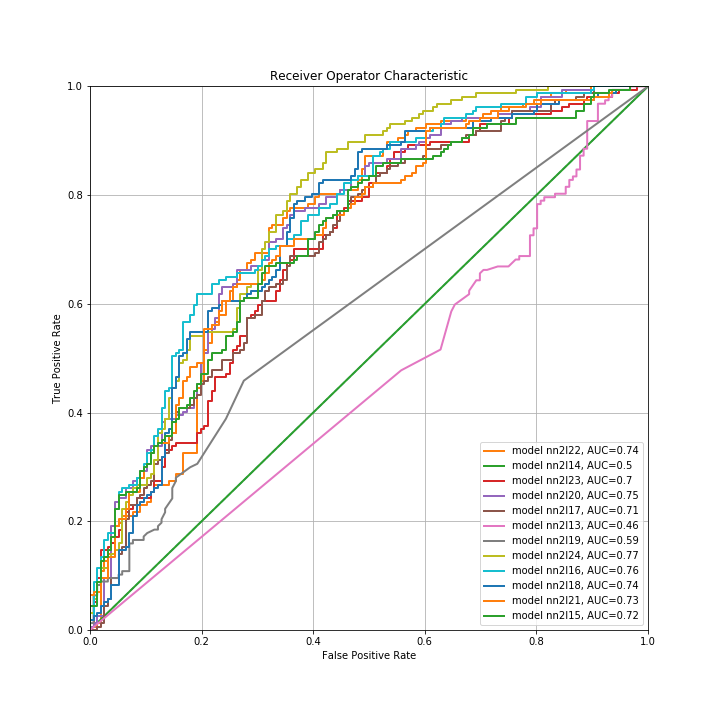
\includegraphics[width=15cm, height=13cm]{../rocNN2L.png}
\end{figure}
\end{center}

\subsection{F{\"u}nf versteckte Schichten}

Die Netze mit f{\"u}nf versteckten Schichten produzierten die weiteste Bandbreite an AUC-Werten. Einerseits produzieren sie den besten Wert, andererseits generiert diese Architektur die meisten uninformativen Modelle. Vier der Modelle weisen einen AUC-Wert nahe bei 0.5 auf. Jedes dieser Modelle enthielt ein einziges Neuron pro Schicht. Das beste der Modelle, \texttt{nn5l36} enthielt f{\"u}nf mal zwanzig Neuronen und produziert einen Wert von 0.8 f{\"u}r die AUC-Metrik. Die Trainingsparameter bestanden aus der geringeren der beiden Lern-Raten (0.005) in Kombination mit einer hohen Anzahl an Epochen.

\begin{center}
\begin{figure}[ht]
\centering
\caption{ROC-Kurve Neuronaler Netze mit f{\"u}nf versteckten Schichten}
\label{rocNN5L}
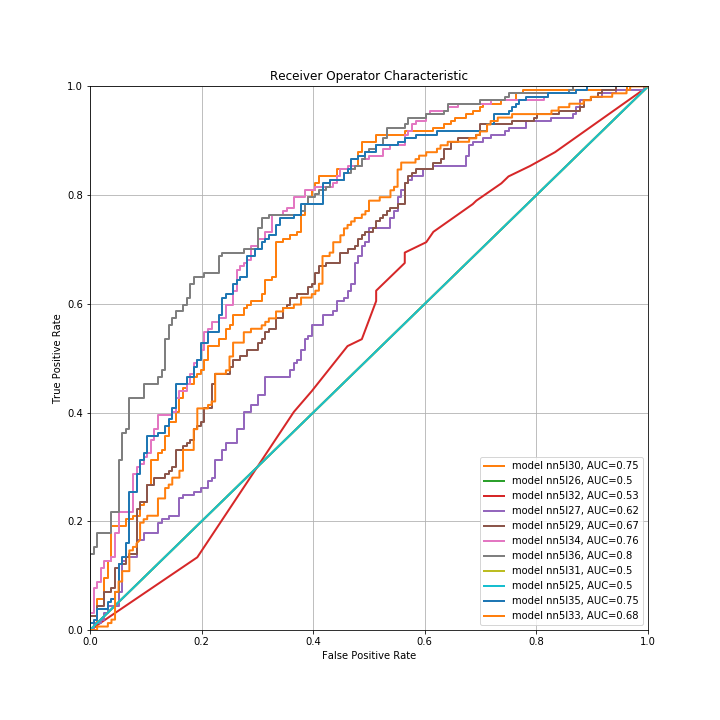
\includegraphics[width=15cm, height=13cm]{../rocNN5L.png}
\end{figure}
\end{center}

\section{Zusammenfassung und kritische W{\"u}rdigung}

Im Verlauf dieser Arbeit haben wir den Datensatz der Creditreform-Datenbank aufbereitet, die betrieblichen Kennzahlen berechnet, verschiedene Architekturen neuronaler Netze vorgestellt und angewandt sowie ausgewertet. F{\"u}r ein simples neuronales Netz haben wir au{\ss}erdem die Einfl{\"u}sse einiger ausgew{\"a}hlter Variablen auf die Ausfallwahrscheinlichkeit visualisiert und interpretiert. Wir haben verschiedene Hyperparameter ausprobiert und die resultierenden Prognosen der neuronalen Netze anhand ihrer AUC-Werte miteinander verglichen. Dabei konnten wir verifizieren, dass die Qualit{\"a}t der Vorhersagen ma{\ss}geblich von der Anzahl der Neuronen pro versteckter Schicht abh{\"a}ngen. Je mehr Neuronen pro Schicht dem Netz zur Verf{\"u}gung stehen, desto besser sind die potentiellen Ergebnisse. Ist die Anzahl der Neuronen hingegen zu gering, besteht die Gefahr des \textit{underfittings}. Erh{\"o}ht man hingegen die Anzahl der Schichten, gestaltet sich der Trainingsprozess zunehmend komplizierter. Die neuronalen Netze mit den f{\"u}nf versteckten Schichten bargen das h{\"o}chste Risiko w{\"a}hrend der Optimierung der Kostenfunktion in einem lokalen Minimum h{\"a}ngen zu bleiben und somit unbrauchbare Prognosen zu liefern. Allerdings lieferten ebenjene Netze auch die besten Ergebnisse, falls der Trainingsprozess erfolgreich durchlaufen wurde.

Eine Bemerkung sei der Generierung von Trainings- und Validierungsdatensatz geg{\"o}nnt. Viele der Beobachtungen innerhalb des Rohdatensatzes wurden nicht verwendet. Eine Alternative zu unserer Vorgehensweise best{\"u}nde darin den Datensatz nach dem Jahr der Beobachtung einzuteilen und den sp{\"a}teren Datensatz zur Validierung zu verwenden(vgl. Chen, 2011). Diese Design-Methode zwingt dem Datensatz jedoch eine zeitliche Struktur auf und wurde hier zugunsten eines zuf{\"a}lligeren Verfahrens verworfen.

\section{Anhang}
\subsection{Code: Hilfsfunktionen}
\lstinputlisting[language=Python]{../utils/generate_configs.py}
\lstinputlisting[language=Python]{../utils/graphs.py}
\lstinputlisting[language=Python]{../utils/roc.py}
\subsection{Code: Datenaufbereitung}
\lstinputlisting[language=Python]{../preprocessing/data_cleaning.py}
\lstinputlisting[language=Python]{../preprocessing/ratios.py}
\subsection{Code: Modelle}
\lstinputlisting[language=Python]{../models/ann.py}
\subsection{Code: Training}
\lstinputlisting[language=Python]{../main.py}


\begin{thebibliography}{9}
\bibitem{altman68}
  Altman, E., (1968), Finantioal Ratios, Discriminant Analysis and the Prediciton of Corporate Bankruptcy. The Journal of Finance, Vol. 23, 4: 589-609.
\bibitem{berk16}
  Berk, J., DeMarzo, P. (2016), Corporate Finance, 4th edition, Harlow, Pearson Education
\bibitem{moro11}
  Chen, S., H{\"a}rdle, W.K., Moro, A.R (2011), Modeling default risk with support vector machines,  Quantitative Finance, 11(1), 135-154.
\bibitem{duda73}
Duda, R. O., Hart, P. E., Stork, D. G. (1973). Pattern Classification. New York: Wiley-Interscience.
\bibitem{miao18}
  Miao, H., Ramchander, S., Ryan, P., Wang, T. (2018), Default prediction models: The role of forward-looking      measures of returns and volatility, Journal of Empirical Finance, 46: 146-162
\bibitem{winkel09}
  Winkelmann, R., Boes, S. (2009): Analysis of Microdata, 2nd edition, 124-128.

\bibitem{Zhang10}
  Zhang, J.L., H{\"a}rdle, W.K. (2010). The Bayesian Additive Classification Tree Applied to Credit Risk Modelling. Computational Statistics and Data Analysis, 54: 1197-1205

\bibitem{scipy}
  Jones, E, Oliphant, T., Peterson, P. (2001), Scipy: open source scientific tools for Python.
\bibitem{matplotlib}
  Hunter, J. D., (2007) Matplotlib: A 2D graphics environment
\bibitem{tensorflow}
Abadi M., Agarwal A., Barham, P., et al. (2015): Large-Scale Machine Learning on Heterogeneous Systems
\bibitem{pandas}
  McKinney, W. (2010): ata Structures for Statistical Computing in Python.
\end{thebibliography}
\end{document}
